\documentclass[12pt,a4paper,titlepage,oneside]{book}
\usepackage[utf8]{inputenc} % para usar utf8
\usepackage{amsmath} % mates
\usepackage[document]{ragged2e} % justificacion de texto
\usepackage{fancyhdr} % un poco de formateo
\usepackage{graphicx} % imagenes

\graphicspath{ {./img/} }

\title{Lenguaje de programación Quartz}
\author{Diego Delgado Barcaiztegui}
\date{26 de Enero del 2021}

\pagestyle{fancy}
\fancyhead{}

\renewcommand{\headrulewidth}{0.2pt}
\renewcommand{\footrulewidth}{0.2pt}

\begin{document}
\maketitle
\tableofcontents
\justify

%\section{Agradecimientos}

%A mi madre y mi padre, que se desviven día a día para darme lo mejor de sí mismos.

%\section{Abstract}
%TODO this shit

\chapter{Autómatas y lenguajes formales}
\begin{center}
\vspace*{3cm}
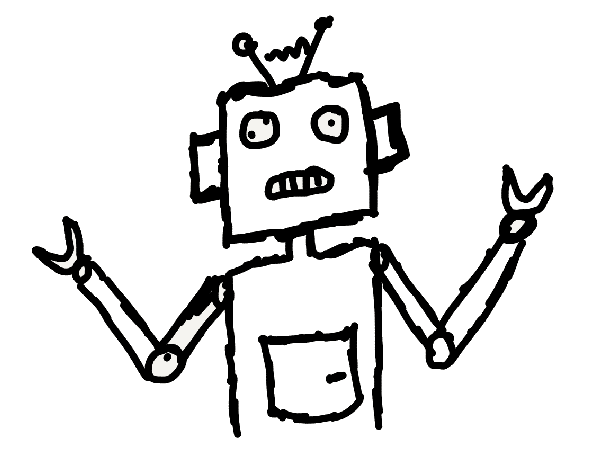
\includegraphics[scale=0.5]{automata}
\end{center}

\newpage

En esta sección vamos a repasar algunos conceptos de teoría de autómatas y lenguajes formales que serán necesarios al momento de definir la especificación del lenguaje de programación Quartz.

\section{Definiciones básicas}

\begin{itemize}

\item \textbf{Alfabeto:} ($\sum$) es un conjunto finito no vacío de símbolos. Por ejemplo $\sum = \{a,b\}$ o $\sum = \{>,<,?\}$.

\item \textbf{Símbolo:} Componente mínimo e indivisible que puede formar parte de una palabra.

\item \textbf{Palabra:} Secuencia finita de símbolos de un alfabeto.

\item \textbf{Longitud de una palabra:} ($|x|$) Cantidad de símbolos que tiene una palabra.

\item \textbf{Palabra vacía: } Se puede representar con $\epsilon$ o $\lambda$. Cumple que $|\lambda| = 0$.

\item \textbf{$\sum^*$:} Conjunto infinito de todas las palabras que se pueden formar con el alfabeto $\sum$, incluyendo $\lambda$. Por ejemplo, teniendo el alfabeto $\sum = \{a, b\}$ entonces $\sum^* = \{\lambda, a, b, aa, bb, abab, abba, ba,...\}$.

\item \textbf{$\sum^+$:} Se define como $\sum^+ = \sum^* - \{\lambda\}$.

\end{itemize}

\section{Lenguajes formales}

Un lenguaje formal L definido sobre el alfabeto $\sum$ se define como $L(\sum) \subset \sum^*$ o más detalladamente $L(\sum) = \{x \in \sum^* |$ x cumple con la definición formal del lenguaje$\}$

Algunos ejemplos pueden ser:

\begin{itemize}

\item $L = \{\} = \emptyset$.
\item $L = \{\in\}$. En este caso es un lenguaje con un elemento: la palabra vacia.
\item $\sum^* =$ lenguaje universal a $\sum$.

\end{itemize}


\end{document}